\section{Untangling feature magnitude and location}
\label{sec-where-info}
The convolutional layers of the network (layers 1-5) preserve the coarse spatial layout of the network's input.
By layer conv-5, the original $227 \times 227$ input image has been progressively downsampled to $6 \times 6$.
The $6 \times 6$ spatial grid in conv-5 encodes the input in a feature map that is computed by 256 filters.
This feature map is also sparse due to the $\max(x, 0)$ non-linearities used in the network (conv-5 is roughly 27\% non-zero; sparsity statistics for all layers are given in Table \ref{table:sparse}).

The network's convolutional layers encode information in terms of (1) which filters have non-zero responses, (2) the magnitudes of those responses, and (3) the spatial locations of the responses.
We will investigate how different filters encode information in Section \ref{sec:grand-mother} (i.e., Is the representation distributed or does it consist of ``grandmother cells''?).
In this section, we experimentally analyze the role of filter response magnitude and spatial location by looking at lesion studies on classification and detection tasks.

\begin{figure}[t!]
\centering
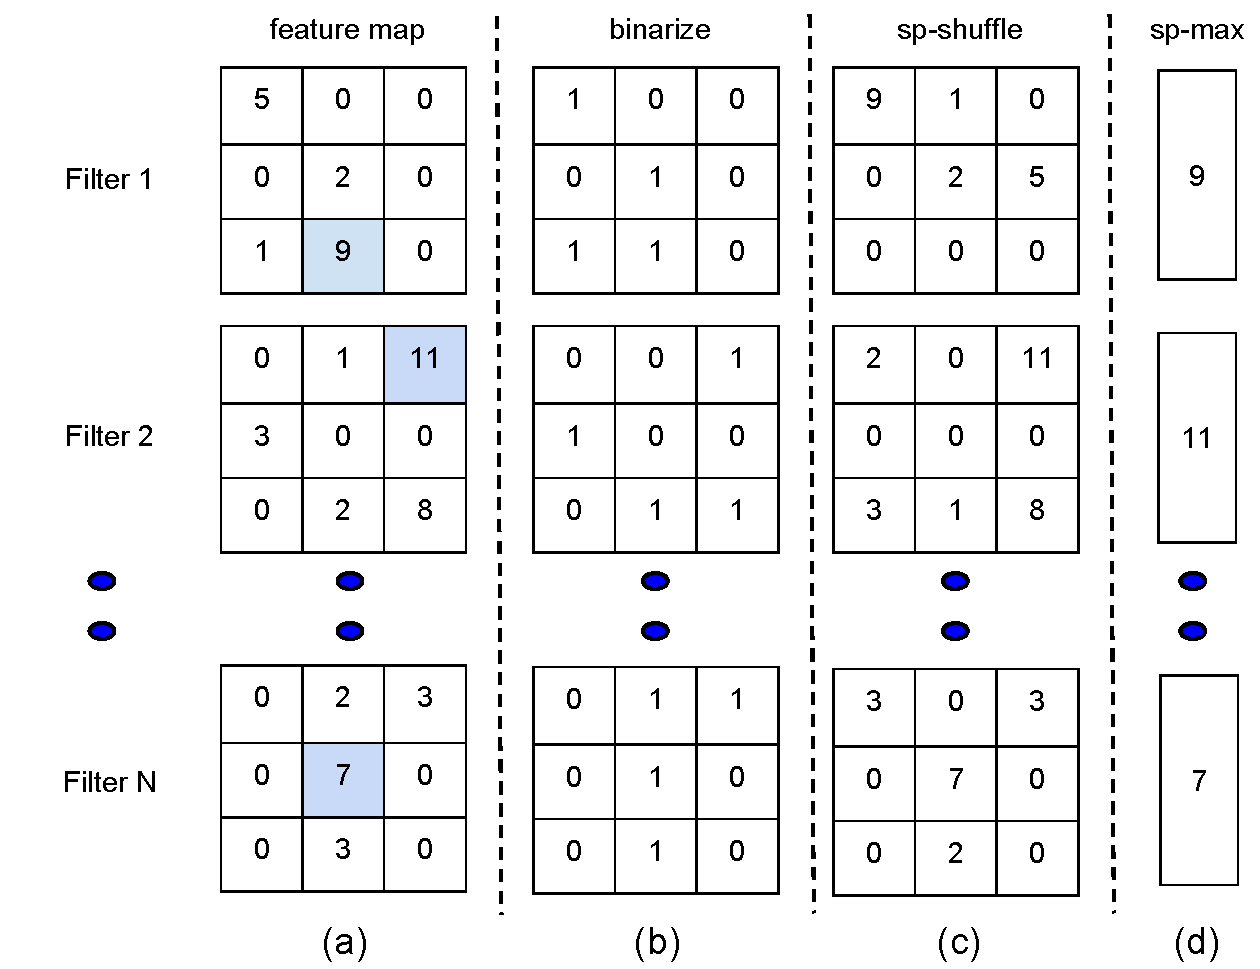
\includegraphics[height=6.5cm]{images/ablation.pdf}
\caption{Illustrations of ablations of feature activation spatial and magnitude information.
See \ref{sub:imp-mag} and \ref{sub:imp-loc} for details.}
  %(a) For illustration, consider the output of a hypothetical layer of size k*k*N (k=3 for convolutional layers and k=1 for FC layers), which has N filters and their responses at k*k spatial locations. Linear SVMs were trained (one for each layer) after vectorizing (i.e. x(:) in matlab) features into a one-dimensional vector of length k*k*N to measure performance of different layers. Next, feature ablations as described below were applied before training SVMs and performance was compared against the un-ablated features. The set of k*k locations for each filter is called its feature map. (b) \textit{spatial-shuffle}(sp-shuffle) -  A random permutation is applied to the set of k*k activations associated with each feature map. Different images see different permutations. (c)\textit{spatial max}(sp-max): For each feature map, the maximum value is selected from the set of k*k activations. (d)\textit{binarization}(bin) Feature dimensions with value $>0$ are set to 1 and others to 0.}
\label{fig:features}
\end{figure}

\subsection{How important is filter response magnitude?}
\label{sub:imp-mag}
\setlength{\tabcolsep}{4pt}
\begin{table}[t!]
\begin{center}
%\caption{Percentage non-zeros (sparsity) in filter responses of various layers of CNN.}
\caption{Percentage non-zeros (sparsity) in filter responses of CNN.}
\label{table:sparse}
\vspace{0.3em}
\scalebox{1}{
\begin{tabular}{c|c|c|c|c|c|c}
conv-1 & conv-2 & conv-3 & conv-4 & conv-5 & fc-6 & fc-7 \\
\hline
$87.5 \pm 4.4$ & $44.5 \pm 4.4$ & $31.8 \pm 2.4$ & $32.0 \pm 2.7$ & $27.7 \pm 5.0$ & $16.1 \pm 3.0$ & $21.6 \pm 4.9$ \\
\end{tabular}}
\end{center}
\end{table}
\setlength{\tabcolsep}{1.4pt}

We can asses the importance of magnitude by setting each filter response $x$ to 1 if $x > 0$ and to $0$ otherwise. This binarization is performed prior to using the responses as features in a linear classifier and leads to loss of information contained in the magnitude of response while still retaining information about which filters fired and where they fired. 
In Tables \ref{table:class-ablation} and \ref{table:det-ablation} we show that binarization leads to a negligible decline in performance for both classification and detection. 

For the fully-connected layers (fc-6 and fc-7) PASCAL image classification performance is nearly identical before and after binarization.
This is a non-trivial property since transforming traditional computer vision features into short (or sparse) binary codes is an active research area. Such codes are important for practical applications in large-scale image retrieval and mobile image analysis \todo{add citations}. Here we observe that sparse binary codes come essentially ``for free'' when using the representations learned in the fully-connected layers.

\subsection{How important is response location?}
\label{sub:imp-loc}
Now we remove spatial information from filter responses while retaining information about their magnitudes. We consider two methods for ablating spatial information from features computed by the convolutional layers (the fully-connected layers do not contain \emph{explicit} spatial information).

The first method (``sp-max'') simply collapses the $p \times p$ spatial map into a single value per feature channel by max pooling. The second method (``sp-shuffle'') retains the original distribution of feature activation values, but scrambles spatial correlations between columns of feature channels. To perform sp-shuffle, we permute the spatial locations in the $p \times p$ spatial map. This permutation is performed independently for each network input (i.e., different inputs undergo different permutations). Columns of filter responses in the same location move together, which preserves correlations between features within each (shuffled) spatial location. These transformations are illustrated in Figure \ref{fig:features}.

For image classification, damaging spatial information leads to a large difference in performance between original and spatially-ablated conv-1 features, but with a gradually decreasing difference for higher layers (Table \ref{table:class-ablation}). 
In fact, the performance of conv-5 after sp-max is close to the original performance. 
This indicates, that a lot of information important for classification is encoded in the activation of the filters and not necessarily in the spatial pattern of their activations. 
However, for detection sp-max (Tables \ref{table:det-ablation}) leads to a large drop in performance. 
This may not be surprising as in contrast to classification, detection requires spatial information precise localization.

\setlength{\tabcolsep}{4pt}
\begin{table}[t!]
\begin{center}
\caption{Location and magnitude ablation study on PASCAL image classification.}
\label{table:class-ablation}
\begin{tabular}{lccccc}
\hline\noalign{\smallskip}
layer & no ablation & binarize & sp-shuffle & sp-max \\
\noalign{\smallskip}
\hline
\noalign{\smallskip}
conv-1 & $25.1 \pm 0.5$ & $17.7 \pm 0.2$ & $15.1 \pm 0.3$ & $25.4 \pm 0.5$  \\ 
conv-2 & $45.3 \pm 0.5$ & $43.0 \pm 0.6$ & $32.9 \pm 0.7$ & $40.1 \pm 0.3$  \\ 
conv-3 & $50.7 \pm 0.6$ & $47.2 \pm 0.6$ & $41.0 \pm 0.8$ & $54.1 \pm 0.5$  \\
conv-4 & $54.5 \pm 0.7$ & $51.5 \pm 0.7$ & $45.2 \pm 0.8$ & $57.0 \pm 0.5$  \\
conv-5 & $65.6 \pm 0.6$ & $60.8 \pm 0.7$ & $59.5 \pm 0.4$ & $62.5 \pm 0.6$  \\
fc-6   & $71.7 \pm 0.3$ & $71.5 \pm 0.4$ &  -             &  -   \\
fc-7   & $74.1 \pm 0.3$ & $73.7 \pm 0.4$ &  -             &  -   \\
\hline
\end{tabular}
\end{center}
\end{table}
\setlength{\tabcolsep}{1.4pt}

\setlength{\tabcolsep}{1pt}
\begin{table}[t!]
\begin{center}
\caption{Ablation study on PASCAL object detection using conv-5 features. Feature binarization leads to negligible drop in performance whereas as sp-max causes a large drop.}
\label{table:det-ablation}
\vspace{0.3em}
\scalebox{0.70}{
\begin{tabular}{l|cccccccccccccccccccc||c}
\noalign{\smallskip}
& aero & bike & bird & boat & bottle & bus & car & cat & chair & cow & table & dog & horse & mbike & person & plant & sheep & sofa & train & tv & mAP \\
\noalign{\smallskip}
\hline
conv-5  & 57.8 & 63.9 & 38.8 & 28.0 & 29.0 & 54.8 & 66.9 & 51.3 & 30.5 & 52.1 & 45.2 & 43.2 & 57.3 & 58.8 & 46.0 & 27.2 & 51.2 & 39.3 & 53.3 & 56.6 & 47.6 \\
binarize & 57.9 & 61.3 & 32.6 & 24.7 & 27.5 & 55.0 & 64.7 & 49.8 & 25.3 & 47.4 & 44.5 & 40.3 & 54.6 & 56.4 & 43.6 & 27.1 & 48.4 & 41.6 & 54.3 & 57.6 & 45.7 \\
sp-max & 35.0 & 38.7 & 17.3 & 16.9 & 13.9 & 38.4 & 45.6 & 29.2 & 11.0 & 20.2 & 21.0 & 23.5 & 27.2 & 37.0 & 20.5 & 7.0 & 30.3 & 13.4 & 28.3 & 32.9 & 25.4 \\
\noalign{\smallskip}
\end{tabular}}
\end{center}
\end{table}
\setlength{\tabcolsep}{1.4pt}
